\emph{Q$^{2}$ADPZ} (\textbf{Q}uite \textbf{A}dvanced \textbf{D}istributed \textbf{P}arallel \textbf{Z}ystem), es un sistema de computaci�n distribuida, multiplataforma y multiusuario para computadores de escritorio no dedicados dentro de una red TCP/IP. El poder de un gran n�mero de computadores ociosos es utilizado por usuarios que pueden ingresar tareas adem�s de monitorear su progreso. La flexibilidad del sistema implica varios modos en que las aplicaciones pueden ser ejecutadas. Tanto los programas de la tareas, los requerimientos de hardware y los archivos de entrada y salida son autom�ticamente manipulados por el sistema. Q$^{2}$ADPZ usa un protocolo de comunicaci�n interno basado en mensajes en formato XML.
\subsubsection{Caracter�sticas}
Los objetivos del dise�o de Q$^{2}$ADPZ son la facilidad de uso para diferentes niveles de conocimiento de los usuarios, operabilidad multiplataforma, arquitectura cliente-maestro-esclavo usando una r�pida comunicaci�n a base de mensajes, modularidad y adaptabilidad, seguridad de los computadores involucrados en el sistema, y sencillez en los procesos de instalaci�n y actualizaci�n.

En Q$^{2}$ADPZ, un peque�o programa (\emph{servicio esclavo}) corre en cada computador de escritorio. Mientras el computador no est� siendo utilizado, el servicio esclavo acepta tareas enviadas por el servidor (\emph{maestro}). El poder de c�mputo disponible es usado para ejecutar la tarea.
\subsubsection{Modos de uso}
El modo b�sico de uso de Q$^{2}$ADPZ es a trav�s de una aplicaci�n de l�nea de comando llamada \emph{cliente universal} y que le permite a los usuarios ingresar el programa a ejecutar. En este ingreso se puede especificar
\begin{itemize}
\item n�mero de ejecuciones del programa,
\item la ruta del ejecutable y los argumentos de l�nea de comando,
\item archivos de entrada y salida,
\item directorios donde residen los archivos,
\item utilidades a ser ejecutadas despu�s de las tareas individuales,
\item tiempo m�ximo asignado para la ejecuci�n de una tarea,
\item el orden en que los grupos de tareas ser�n ejecutados,
\item requerimientos de hardware (espacio en disco, memoria, velocidad y tipo de CPU) y software (sistema operativo y programas instalados).
\end{itemize}

Estos par�metros de configuraci�n son guardados en un archivo en formato XML. El ejecutable puede ser obtenido desde el disco local o descargado desde alguna direcci�n URL. Los archivos de entrada y salida son transferidos a los esclavos usando un servidor web dedicado a los datos.

Cada ejecuci�n corresponde a una tarea - la unidad de c�mputo m�s peque�a en Q$^{2}$ADPZ. Las tareas son agrupadas en trabajos - identificadas por un identificador y un nombre. El sistema permite la operaci�n de control sobre tareas, trabajos y usuarios. Usuarios avanzados pueden crear el archivo de configuraci�n manualmente o generarlo autom�ticamente.

Usuarios a�n m�s avanzados pueden prescindir del cliente universal y programar su propia \emph{aplicaci�n cliente}\footnote{user client application} que se comunique directamente con el maestro, permitiendo ingresar tareas din�micamente. Finalmente, los usuarios pueden programar sus propias \textit{bibliotecas esclavas}\footnote{user slave library} que en casos espec�ficos son, por lo general, m�s r�pidas que los programas ejecutables.


\subsubsection{Arquitectura}
El sistema consiste en un proceso central llamado \emph{maestro}, un n�mero variable de procesos en diferentes computadores de una red llamados \emph{esclavos} y un n�mero de procesos \emph{cliente} que generan tareas agrupadas en trabajos. En la figura \ref{fig:image01} se grafica este esquema.
\begin{figure}
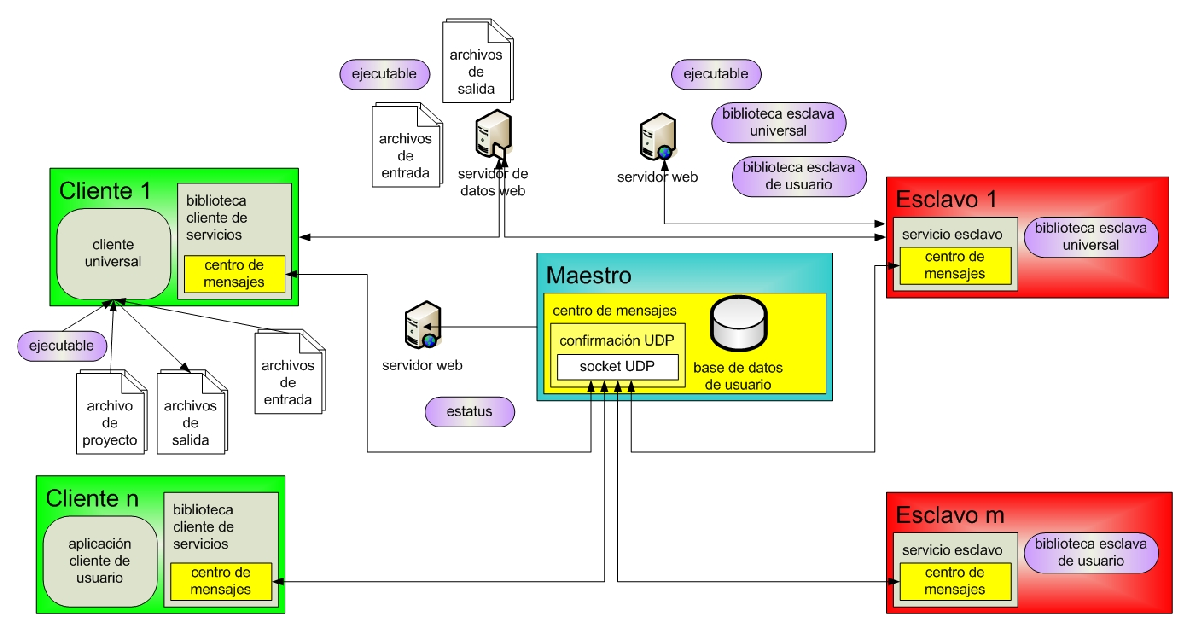
\includegraphics[width=\textwidth]{images/image01.eps}
\caption{La arquitectura de Q$^2$ADPZ}
\label{fig:image01}
\end{figure}
El componente esclavo corre como un proceso permanente. Su rol principal es notificar al \emph{maestro} sobre su estado y sus recursos disponibles. Otro rol que posee es lanzar una aplicaci�n, consecuencia de una petici�n del maestro. La aplicaci�n, en la forma de una biblioteca, ejecutable o programa interpretado, es transferida desde el servidor de acuerdo a la descripci�n de la tarea, entonces es ejecutada con los argumentos de l�nea de comando especificadas en dicha descripci�n.

Al momento en que un esclavo recibe una tarea, en primera instancia descarga el ejecutable o programa interpretado desde un repositorio autom�tico de datos (implementado sobre un servidor web en Perl), o desde una direcci�n URL. Luego, el esclavo procede a descargar y preparar todos los archivos de entrada requeridos. Despu�s que el ejecutable o programa interpretado termina, los archivos de salida generados son subidos al repositorio web para ser posteriormente obtenidos por el cliente que cre� la tarea.

El maestro adem�s escucha a todos los esclavos y de esta forma tiene una visi�n general de todos los recursos disponibles en el sistema. El maestro acepta peticiones de tareas de los clientes y le asigna los nodos (esclavos) m�s adecuados. Adem�s de esto, el maestro permite reservar nodos: los clientes son notificados despu�s de que los recursos se encuentren disponibles.

El cliente consiste en una aplicaci�n que usa una biblioteca cliente de servicios. Esta biblioteca provee una API C++ para la comunicaci�n con el maestro, permitiendo controlar y comenzar trabajos y tareas, adem�s de obtener los resultados de �stos. Los usuarios pueden utilizar la API directamente en sus aplicaciones o usar un cliente universal que ingresa y controla las tareas en base a un archivo de especificaci�n en formato XML.

\subsubsection{Comunicaci�n}
La comunicaci�n es un aspecto primordial de todo sistema que funcione sobre una red. En esta secci�n se describe el protocolo de comunicaci�n entre los diferentes elementos del sistema. Qt4 dispone de m�ltiples clases y tipos de datos que facilitan la implementaci�n de la comunicaci�n y que son nombrados en esta secci�n. Para obtener una descripci�n m�s detallada de estos, se solicita al lector revisar la documentaci�n de Qt4 disponible en l�nea\cite{qtdocpage}. En esta secci�n se utiliza el mecanismo de descripci�n de mensajes explicado en el anexo \ref{anexo:definicion_mensaje}. 
\subsection{Protocolo cliente-maestro}
La comunicaci�n entre el cliente y el maestro toma como base el protocolo TCP. El maestro funciona como servidor TCP sobre un puerto en espec�fico. Cuando un programa cliente hace una petici�n\footnote{las peticiones corresponden a las diferentes acciones que el usuario puede acceder mediante el cliente que se encuentran descritas en la secci�n \ref{ref:arquitectura_usuarios}}, establece una conexi�n al maestro y seg�n la petici�n que haya solicitado son los mensajes que intercambiar�n. Todos los intercambios de mensajes de las diferentes peticiones parten con un marco de comunicaci�n destinado a la autenticaci�n del usuario que determina si el usuario est� habilitado para hacer la acci�n que establece en la petici�n. Si despu�s de esto se determina que el usuario est� habilitado para desarrollar la acci�n, entonces el intercambio de mensajes prosigue seg�n la petici�n que se haya efectuado. 
\subsubsection{Marco de autenticaci�n}
\begin{itemize}
\item \textbf{Diagrama :}\\
\begin{tabular}{ l l}
\texttt{| quint8 acc | QString user | QString pass |}&\texttt{cliente>maestro}\\
\texttt{| quint8 resp |}&\texttt{cliente<maestro}
\end{tabular}
\item \textbf{Descripci�n :} Este marco de comunicaci�n sirve para determinar si el usuario tiene permitido ejecutar una acci�n. \item \textbf{Campos:}
\begin{itemize}
\item \textbf{acc:} Valor num�rico que codifica la acci�n a ejecutar por el cliente.
\item \textbf{user:} Nombre de usuario
\item \textbf{pass:} Contrase�a de usuario.
\item \textbf{rest:} Valor num�rico que codifica la respuesta del maestro.
\end{itemize}
\end{itemize}
\subsubsection{Marco agregar trabajo}
\begin{itemize}
\item \textbf{Diagrama :}\\
\begin{tabular}{ l l}
\texttt{| QByteArray data |}&\texttt{cliente>maestro}\\
\texttt{| qint32 id |}&\texttt{cliente<maestro}
\end{tabular}
\item \textbf{Descripci�n :} Este marco de comunicaci�n sirve para agregar un trabajo al maestro.
\item \textbf{Campos:}
\begin{itemize}
\item \textbf{data:} Datos del archivo de especificaci�n del trabajo comprimidos con el algoritmo gzip.
\item \textbf{id:} Identificador que el maestro le asoci� al trabajo.
\end{itemize}
\end{itemize}
\subsubsection{Marco agregar trabajo local}
\begin{itemize}
\item \textbf{Diagrama :}\\
\begin{tabular}{ l l}
\texttt{| QString path |}&\texttt{cliente>maestro}\\
\texttt{| qint32 id |}&\texttt{cliente<maestro}
\end{tabular}
\item \textbf{Descripci�n :} Este marco de comunicaci�n sirve para agregar un trabajo al maestro que se encuentra en el mismo computador. Con este m�todo se ahorra el tiempo de transferencia por red.
\item \textbf{Campos:}
\begin{itemize}
\item \textbf{path:} Ruta del archivo de especificaci�n del trabajo.
\item \textbf{id:} Identificador que el maestro le asoci� al trabajo.
\end{itemize}
\end{itemize}
\subsubsection{Marco borrar trabajo}
\begin{itemize}
\item \textbf{Diagrama :}\\
\begin{tabular}{ l l}
\texttt{| qint32 id |}&\texttt{cliente>maestro}
\end{tabular}
\item \textbf{Descripci�n :} Este marco de comunicaci�n se usa cuando se borra un trabajo.
\item \textbf{Campos:}
\begin{itemize}
\item \textbf{id:} Identificador del trabajo a borrar.
\end{itemize}
\end{itemize}
\subsubsection{Marco obtener informaci�n de trabajo}
\begin{itemize}
\item \textbf{Diagrama :}\\
\begin{tabular}{ l l}
\texttt{| qint32 id |}&\texttt{cliente>maestro}\\
\texttt{| qint32 id | QString user | qint32 comp | qint32 total |}&\texttt{cliente<maestro}
\end{tabular}
\item \textbf{Descripci�n :} Este marco de comunicaci�n se usa cuando se obtiene informaci�n sobre un trabajo.
\item \textbf{Campos:}
\begin{itemize}
\item \textbf{id:} Identificador del trabajo.
\item \textbf{user:} Usuario due�o del trabajo.
\item \textbf{comp:} N�mero de tareas completados.
\item \textbf{total:} N�mero de total de tareas del trabajo.
\end{itemize}
\end{itemize}
\subsubsection{Marco obtener resultados de trabajo}
\begin{itemize}
\item \textbf{Diagrama :}\\
\begin{tabular}{ l l}
\texttt{| qint32 id |}&\texttt{cliente>maestro}\\
\texttt{| QByteArray data |}&\texttt{cliente<maestro}
\end{tabular}
\item \textbf{Descripci�n :} Este marco de comunicaci�n se usa cuando se obtiene los resultados de un trabajo.
\item \textbf{Campos:}
\begin{itemize}
\item \textbf{id:} Identificador del trabajo.
\item \textbf{data:} Datos binarios comprimidos por gzip de los resultados del trabajo.
\end{itemize}
\end{itemize}
\subsubsection{Marco obtener resultados de trabajo local}
\begin{itemize}
\item \textbf{Diagrama :}\\
\begin{tabular}{ l l}
\texttt{| qint32 id |}&\texttt{cliente>maestro}\\
\texttt{| QString path |}&\texttt{cliente<maestro}
\end{tabular}
\item \textbf{Descripci�n :} Este marco de comunicaci�n se usa cuando se obtiene los resultados de un trabajo cuando el maestro se encuentra en la misma m�quina.
\item \textbf{Campos:}
\begin{itemize}
\item \textbf{id:} Identificador del trabajo.
\item \textbf{path:} Ruta del archivo de resultados en el computador.
\end{itemize}
\end{itemize}
\subsubsection{Marco listar trabajos}
\begin{itemize}
\item \textbf{Diagrama :}\\
\begin{tabular}{ l l}
\texttt{| qint32 id\_1 | QString user\_1 |}&\texttt{cliente<maestro}\\
\texttt{| qint32 id\_2 | QString user\_2 |}&\texttt{cliente<maestro}\\
\texttt{| qint32 id\_n | QString user\_n |}&\texttt{cliente<maestro}\\
\end{tabular}
\item \textbf{Descripci�n :} Este marco de comunicaci�n se usa cuando se desea obtener la lista de trabajos que hay en el sistema.
\item \textbf{Campos:}
\begin{itemize}
\item \textbf{id\_x:} Identificador del trabajo x.
\item \textbf{user\_x:} Usuario due�o del trabajo x.
\end{itemize}
\end{itemize}
\subsubsection{Marco borrar tarea}
\begin{itemize}
\item \textbf{Diagrama :}\\
\begin{tabular}{ l l}
\texttt{| qint32 job | qint32 id |}&\texttt{cliente>maestro}\\
\end{tabular}
\item \textbf{Descripci�n :} Este marco de comunicaci�n se usa cuando se desea borrar de una tarea en espec�fico.
\item \textbf{Campos:}
\begin{itemize}
\item \textbf{job:} Identificador del trabajo.
\item \textbf{id:} Identificador de la tarea.
\end{itemize}
\end{itemize}
\subsubsection{Marco obtener informaci�n de tarea}
\begin{itemize}
\item \textbf{Diagrama :}\\
\begin{tabular}{ l l}
\texttt{| qint32 job | qint32 id |}&\texttt{cliente>maestro}\\
\texttt{| qint32 id | QString prog | QString args | QString ret |}&\texttt{cliente<maestro}\\
\end{tabular}
\item \textbf{Descripci�n :} Este marco de comunicaci�n se usa cuando se desea obtener informaci�n sobre una tarea.
\item \textbf{Campos:}
\begin{itemize}
\item \textbf{job:} Identificador del trabajo.
\item \textbf{id:} Identificador de la tarea.
\item \textbf{prog:} Nombre del programa a ajecutar por la tarea.
\item \textbf{args:} Argumentos de l�nea de comando de la tarea.
\item \textbf{ret:} Lista de archivos a recuperar por la ejecuci�n de la tarea separador por coma (,).
\end{itemize}
\end{itemize}
\subsubsection{Marco listar tareas}
\begin{itemize}
\item \textbf{Diagrama :}\\
\begin{tabular}{ l l}
\texttt{| qint32 job |}&\texttt{cliente>maestro}\\
\texttt{| qint32 id\_1 | QString prog\_1 |}&\texttt{cliente<maestro}\\
\texttt{| qint32 id\_2 | QString prog\_2 |}&\texttt{cliente<maestro}\\
\texttt{| qint32 id\_n | QString prog\_n |}&\texttt{cliente<maestro}\\
\end{tabular}
\item \textbf{Descripci�n :} Este marco de comunicaci�n se usa cuando se desea obtener la lista de tareas de un trabajo.
\item \textbf{Campos:}
\begin{itemize}
\item \textbf{job:} Identificador del trabajo.
\item \textbf{id\_x:} Identificador de la tarea x.
\item \textbf{prog\_x:} Nombre del programa a ajecutar por la tarea x.
\end{itemize}
\end{itemize}
\subsubsection{Marco agregar grupo}
\begin{itemize}
\item \textbf{Diagrama :}\\
\begin{tabular}{ l l}
\texttt{| QString group | QString url | QString user |}&\texttt{cliente>maestro}\\
\end{tabular}
\item \textbf{Descripci�n :} Este marco de comunicaci�n se usa cuando se desea agregar un grupo.
\item \textbf{Campos:}
\begin{itemize}
\item \textbf{group:} Nombre de grupo.
\item \textbf{url:} Direcci�n URL con la lista de p�ginas a mostrar por el salvapantallas.
\item \textbf{user:} Usuario due�o del grupo.
\end{itemize}
\end{itemize}
\subsubsection{Marco cambiar grupo}
\begin{itemize}
\item \textbf{Diagrama :}\\
\begin{tabular}{ l l}
\texttt{| QString group | QString url |}&\texttt{cliente>maestro}\\
\end{tabular}
\item \textbf{Descripci�n :} Este marco de comunicaci�n se usa cuando se desea cambiar la URL con la lista de p�ginas a mostrar por el salvapantallas.
\item \textbf{Campos:}
\begin{itemize}
\item \textbf{group:} Nombre de grupo.
\item \textbf{url:} Direcci�n URL con la lista de p�ginas a mostrar  por el salvapantallas.
\end{itemize}
\end{itemize}
\subsubsection{Marco borrar grupo}
\begin{itemize}
\item \textbf{Diagrama :}\\
\begin{tabular}{ l l}
\texttt{| QString group |}&\texttt{cliente>maestro}\\
\end{tabular}
\item \textbf{Descripci�n :} Este marco de comunicaci�n se usa cuando se desea borrar un grupo.
\item \textbf{Campos:}
\begin{itemize}
\item \textbf{group:} Nombre de grupo.
\end{itemize}
\end{itemize}
\subsubsection{Marco obtener informaci�n de grupo}
\begin{itemize}
\item \textbf{Diagrama :}\\
\begin{tabular}{ l l}
\texttt{| QString group |}&\texttt{cliente>maestro}\\
\texttt{| QString url | QString user |}&\texttt{cliente<maestro}\\
\end{tabular}
\item \textbf{Descripci�n :} Este marco de comunicaci�n se usa cuando se desea obtener informaci�n sobre un grupo.
\item \textbf{Campos:}
\begin{itemize}
\item \textbf{group:} Nombre de grupo.
\item \textbf{url:} Direcci�n URL con la lista de p�ginas a mostrar por el salvapantallas.
\item \textbf{user:} Usuario due�o del grupo.
\end{itemize}
\end{itemize}
\subsubsection{Marco obtener lista de grupos}
\begin{itemize}
\item \textbf{Diagrama :}\\
\begin{tabular}{ l l}
\texttt{| QString group\_1 |}&\texttt{cliente<maestro}\\
\texttt{| QString group\_2 |}&\texttt{cliente<maestro}\\
\texttt{| QString group\_n |}&\texttt{cliente<maestro}
\end{tabular}
\item \textbf{Descripci�n :} Este marco de comunicaci�n se usa cuando se desea obtener la lista de grupos existentes en el sistema.
\item \textbf{Campos:}
\begin{itemize}
\item \textbf{group\_x:} Nombre del grupo x.
\end{itemize}
\end{itemize}
\subsubsection{Marco agregar usuario}
\begin{itemize}
\item \textbf{Diagrama :}\\
\begin{tabular}{ l l}
\texttt{| QString user | QString pass |}&\texttt{cliente>maestro}
\end{tabular}
\item \textbf{Descripci�n :} Este marco de comunicaci�n se usa cuando se desea agregar un usuario al sistema.
\item \textbf{Campos:}
\begin{itemize}
\item \textbf{user:} Nombre de usuario.
\item \textbf{pass:} Contrase�a de usuario.
\end{itemize}
\end{itemize}
\subsubsection{Marco cambiar contrase�a de usuario}
\begin{itemize}
\item \textbf{Diagrama :}\\
\begin{tabular}{ l l}
\texttt{| QString pass |}&\texttt{cliente>maestro}
\end{tabular}
\item \textbf{Descripci�n :} Este marco de comunicaci�n se usa cuando se desea cambiar la contrase�a del usuario.
\item \textbf{Campos:}
\begin{itemize}
\item \textbf{pass:} Contrase�a de usuario.
\end{itemize}
\end{itemize}
\subsubsection{Marco borrar usuario}
\begin{itemize}
\item \textbf{Diagrama :}\\
\begin{tabular}{ l l}
\texttt{| QString user |}&\texttt{cliente>maestro}
\end{tabular}
\item \textbf{Descripci�n :} Este marco de comunicaci�n se usa cuando se desea borrar un usuario.
\item \textbf{Campos:}
\begin{itemize}
\item \textbf{user:} Nombre de usuario a borrar.
\end{itemize}
\end{itemize}
\subsubsection{Marco obtener informaci�n de usuario}
\begin{itemize}
\item \textbf{Diagrama :}\\
\begin{tabular}{ l l}
\texttt{| QString user |}&\texttt{cliente>maestro}\\
\texttt{| QString pass |}&\texttt{cliente<maestro}
\end{tabular}
\item \textbf{Descripci�n :} Este marco de comunicaci�n se usa cuando se desea obtener la contrase�a del usuario.
\item \textbf{Campos:}
\begin{itemize}
\item \textbf{user:} Nombre de usuario.
\item \textbf{pass:} Contrase�a del usuario.
\end{itemize}
\end{itemize}
\subsubsection{Marco obtener lista de usuarios}
\begin{itemize}
\item \textbf{Diagrama :}\\
\begin{tabular}{ l l}
\texttt{| QString user\_1 |}&\texttt{cliente<maestro}\\
\texttt{| QString user\_2 |}&\texttt{cliente<maestro}\\
\texttt{| QString user\_n |}&\texttt{cliente<maestro}
\end{tabular}
\item \textbf{Descripci�n :} Este marco de comunicaci�n se usa cuando se desea obtener la lista de usuarios,
\item \textbf{Campos:}
\begin{itemize}
\item \textbf{user\_x:} Nombre de usuario.
\end{itemize}
\end{itemize}
\subsubsection{Marco reiniciar esclavo}
\begin{itemize}
\item \textbf{Diagrama :}\\
\begin{tabular}{ l l}
\texttt{| QString id |}&\texttt{cliente>maestro}
\end{tabular}
\item \textbf{Descripci�n :} Este marco de comunicaci�n se usa cuando se desea reiniciar un esclavo del sistema.
\item \textbf{Campos:}
\begin{itemize}
\item \textbf{id:} Identificador de esclavo a reiniciar.
\end{itemize}
\end{itemize}
\subsubsection{Marco obtener informaci�n de esclavo}
\begin{itemize}
\item \textbf{Diagrama :}\\
\begin{tabular}{ l l}
\texttt{| qint32 id |}&\texttt{cliente>maestro} \\
\texttt{| qint32 id | QString ip | qint32 port | quint8 prior }&\\
\texttt{| QString last | qint32 cur | qint32 total | QString group |}&\texttt{cliente<maestro}
\end{tabular}
\item \textbf{Descripci�n :} Este marco de comunicaci�n se usa cuando se desea obtener informaci�n sobre un esclavo.
\item \textbf{Campos:}
\begin{itemize}
\item \textbf{id:} Identificador de esclavo.
\item \textbf{ip:} Direcci�n IP del esclavo.
\item \textbf{port:} Puerto del esclavo.
\item \textbf{prior:} Prioridad del esclavo codificada num�ricamente.
\item \textbf{last:} Fecha y hora de la �ltima actualizaci�n del esclavo.
\item \textbf{cur:} N�mero de tareas que el esclavo tiene en ejecuci�n.
\item \textbf{total:} N�mero m�ximo de tareas que el esclavo soporta simultaneamente.
\item \textbf{group:} Grupo al que pertence el esclavo.
\end{itemize}
\end{itemize}
\subsubsection{Marco obtener lista de esclavos}
\begin{itemize}
\item \textbf{Diagrama :}\\
\begin{tabular}{ l l}
\texttt{| qint32 id\_1 | QString ip\_1 | qint32 port\_1 | }&\texttt{cliente<maestro}\\
\texttt{| qint32 id\_2 | QString ip\_2 | qint32 port\_2 | }&\texttt{cliente<maestro}\\
\texttt{| qint32 id\_n | QString ip\_n | qint32 port\_n | }&\texttt{cliente<maestro}
\end{tabular}
\item \textbf{Descripci�n :} Este marco de comunicaci�n se usa cuando se desea obtener la lista de esclavo que se encuentran conectados al sistema.
\item \textbf{Campos:}
\begin{itemize}
\item \textbf{id\_x:} Identificador de esclavo x.
\item \textbf{ip\_x:} Direcci�n IP del esclavo x.
\item \textbf{port\_x:} Puerto del esclavo x.
\end{itemize}
\end{itemize}
\subsection{Protocolo maestro-esclavo}\label{ref:com_maestro_esclavo}
La comunicaci�n entre el programa maestro y el programa esclavo es la m�s compleja de todo el sistema. Esto es a causa de la gran cantidad de programas esclavos con la que el programa maestro debe estar comunicado, y por la necesidad que esta comunicaci�n pase a trav�s de NATs. El protocolo base a utilizar es UDP, que se eligi� ante su alternativa TCP, porque es un protocolo liviano que disminuye la carga presente en la red del sistema. Adem�s la t�cnica elegida para superar el problema sucitado por los NATs (descrita en la pr�xima parte) recomienda el uso de UDP para esto. Sin embargo, UDP implica problemas anexos, como el hecho que no hay control del orden de llegada de los mensajes o si realmente llegaron a su destino. Todos estos inconvenientes y sus soluciones son descritos  a continuaci�n.
\subsubsection{NAT}
Es com�n que las redes locales de peque�as compa��as tengan solo una salida a una red superior como internet, en palabras m�s t�cnicas, todos los computadores tienen asociados una IP interna diferente, pero en la red externas todos comparten la misma direcci�n IP, y esto sucede gracias a NAT. NAT (Traducci�n de Direcciones de Red)\cite{nat} es un mecanismo que permite que direcciones con un puerto interno sean mapeadas con la direcci�n externa m�s un puerto. En la figura \ref{fig:image21} se grafica este mecanismo. Pero como se puede intuir, no hay suficientes combinaciones de direcciones externas con puertos que puedan abarcar todas las combinaciones de direcciones internas con puertos, por eso, NAT asume que no todas estas combinaciones van a estar siendo utilizadas al mismo tiempo y las que combinaciones que terminen de usarse expiran y quedan disponibles para que otra m�quina pueda establecer una conexi�n externa. Pero esto implica un problema con aplicaciones que necesitan una conexi�n permanente ya que eventualmente la direcci�n que antes estaba asignada a una m�quina, en otra ocasi�n puede no estarlo, o estarlo a una m�quina diferente. La mayor�a de los firewall y cortafuegos en la actualidad son NATs lo que hace que el problema no sea algo que se pueda obviar facilmente y menos cuando uno quiere incluir la mayor cantidad de computadores de una red. Sin ir m�s lejos, dentro de la Universidad de Concepci�n, la subred del laboratorio de redes del DIICC usa este mecanismo para sus computadores.  A continuaci�n se describe la soluci�n para superar esta problem�tica.
\begin{figure}
\begin{center}
\includegraphics[width=0.7\textwidth]{images/image21.eps}
\end{center}
\caption{Esquema del funcionamiento de un NAT}
\label{fig:image21}
\end{figure}
\subsubsection{UDP Hole Punching}
\emph{UDP hole punching}\cite{udpholepunching} es una t�cnica para poder comunicar m�quinas que est�n detr�s de NATs lo que hace que ambos no puedan acceder al otro directamente. Esta t�cnica es ampliamente utilizada por diversos protocolos existentes en la actualidad que van desde protocolos de juegos en l�nea, hasta de conocidas aplicaciones como \emph{Skype}\cite{skypepage}.\\
Para explicar la t�cnica se deben tener en cuenta tres entidades que se nombran a continuaci�n:
\begin{itemize}
\item Un servidor \textbf{S} que registre las direcciones IP y los puertos UDP por los cuales los clientes se conectan a �l.
\item Dos clientes \textbf{A} y \textbf{B} que se comuniquen por el protocolo UDP.
\end{itemize}
Ahora los pasos de la t�cnica se nombran a continuaci�n :
\begin{enumerate}
\item \textbf{A} no sabe como alcanzar a \textbf{B}, entonces \textbf{A} pide a \textbf{S} ayuda para establecer una conexi�n UDP con \textbf{B}.
\item \textbf{S} env�a a \textbf{A} un mensaje conteniendo la direcci�n y puerto UDP registrados de \textbf{B}. Al mismo tiempo \textbf{S} env�a a \textbf{B} la direcci�n y puerto UDP de \textbf{A}.
\item Con ambos cliente conociendo las direcciones y puerto del otro. Entonces pueden establecer la conexi�n.
\end{enumerate}
La t�cnica funciona porque cuando los clientes se conectan al servidor, este almancena la direcci�n y puerto que el NAT a asignado para la comunicaci�n (si es que �ste esta presente). Por eso comunicandose con las direcci�n y puerto ofrecidos por el servidor, los clientes pueden acceder el uno al otro. El procedimiento se ilustra en la figura \ref{fig:image22}.
\begin{figure}
\begin{center}
\includegraphics[width=\textwidth]{images/image22.eps}
\end{center}
\caption{El proceso de UDP hole punching}
\label{fig:image22}
\end{figure}
Otro aspecto a considerar es que las asignaciones de direcciones y puertos que hacen los NATs caducan despues de un tiempo, por eso hay que enviar paquetes de comunicaci�n peri�dicamente con el fin que la direcci�n y puerto continuen asignados para el mismo computador.\\
En el cluster virtual no se implementa est� t�cnica exactamente, ya que no hay conexi�n entre clientes, ac� simplemente se necesita de un \emph{medio hole punching}, es decir, que el servidor pueda acceder al cliente y sea capaz de mantener su conexi�n, donde el servidor y el cliente ser�an el programa maestro y el esclavo respectivamente.
\subsubsection{Dando fiabilidad a la comunicaci�n UDP}
Como se dijo anteriormente, UDP no es un protocolo fiable, ya que no provee mecanismos que permitan cerciorarse que un mensaje a llegado adecuadamente. Por eso, el dise�o del protocolo debe considerar este problema. Para superar esto, se crearon unos elementos llamados \emph{repetidores}. Estos elementos son implementados como clases que env�an indefinidamente un paquete UDP hasta que reciben un paquete UDP de notificaci�n de recepci�n del mensaje por el receptor. Este mecanismo asegura que si un mensaje se pierde en el env�o desde el emisor al receptor o viceversa, pueda enviarse nuevamente hasta que una comunicaci�n se complete. En la figura \ref{fig:image26} se ilustra el funcionamiento de los repetidores. La mayor�a de los paquetes UDP que usa el sistema son de un tama�o de 15 bytes con un m�ximo de 400 bytes. Los repetidores reenv�an el paquete cada 10 segundos lo que en el peor de los casos significa una tasa de transferencia 40 Bps\footnote{Bytes por segundo} (400 bytes cada 10 segundos). En el caso que tuvieramos 100 esclavos reci�n estar�amos presente a un flujo de red de aproximadamente 4kBps\footnote{kiloBytes por segundo}, tasa que tan solo representa el 0.032\% de la capacidad de transferencia de una intranet convencional de 12.5MBps\footnote{100 Mbps}.
\begin{figure}
\begin{center}
\includegraphics[width=0.7\textwidth]{images/image26.eps}
\end{center}
\caption{Funcionamiento de los repetidores UDP}
\label{fig:image26}
\end{figure}
\subsubsection{Transferencia de archivos mediante UDP}
Otro aspecto importante para el sistema es la transferencia de archivos. Como se ha reiterado UDP es un sistema poco confiable, pero parte del problema se ha solucionado con la implementaci�n de repetidores. Sin embargo, los paquetes UDP tienen un tama�o m�ximo destinado a los datos, que si bien es suficiente para enviar peque�os mensajes, no lo es para enviar un archivo completo. Por eso un archivo debe ser particionado y enviados en peque�os paquetes. En la figura \ref{fig:image28} se ilustra el mecanismo de transferencia de archivos por partes. Cada parte es enviada por un paquete llamado \texttt{send} mediante un repetidor que se terminado cuando recibe un paquete de notificaci�n \texttt{sendack} y crea un nuevo repetidor con el paquete que corresponde a la parte siguiente del archivo. Pero tal como se muestra el esquema no es suficiente para asegurar la transferencia del archivo ya que los repetidores aseguran que el emisor sepa que el mensaje enviado a llegado, pero no que el receptor sepa que llego el mensaje de notificaci�n. Este problema se puede ejemplificar en el siguiente caso:
\begin{figure}
\begin{center}
\includegraphics[width=0.7\textwidth]{images/image28.eps}
\end{center}
\caption{Mecanismo de transferencia de archivos mediante UDP}
\label{fig:image28}
\end{figure}
\begin{enumerate}
\item El receptor recibe el paquete de la parte 1 del archivo.
\item El receptor env�a el paquete de notificaci�n de que lo ha recibido.
\item El paquete de notificaci�n se pierde en la red.
\item Como el emisor no ha recibido un paquete de notificaci�n, entonces el repetidor env�a nuevamente el paquete de la parte 1.
\end{enumerate}
En este caso el receptor es incapaz de discriminar si el �ltimo paquete que a enviado el emisor es el de la parte 1 por la perdida del paquete de notificaci�n, o si es el de la parte 2 en caso que el paquete de notificaci�n a llegado. Para solucionar esto basta con enumerar los paquetes con el fin de que el receptor pueda discrimar en el caso anteriormente mencionado. Generalmente las transferecias de archivos dentro del sistema est�n asociadas a una tarea en espec�fica. Como el maestro maneja las trasnferencias de m�ltiples tareas a la vez, es necesario agregar al paquete identificadores que lo asocien a una tarea en espec�fico. Con todas est�s consideraciones el formato del paquete \texttt{send} queda de la siguiente forma :
\begin{itemize}
\item \textbf{Diagrama :}\\
\begin{tabular}{ l}
\texttt{| quint8 tipo | qint32 id | qint32 job |}\\
\texttt{| qint32 task | qint32 num | QByteArray data |}
\end{tabular}
\item \textbf{Campos:}
\begin{itemize}
\item \textbf{tipo:} Identificador de tipo de paquete, este valor siempre es 6.
\item \textbf{id:} Identificador del esclavo. Independiente si la transferencia es desde o hacia el esclavo.
\item \textbf{job:} Identificador del trabajo al que asociado el archivo.
\item \textbf{task:} Identificador de la tarea a la que asociado el archivo.
\item \textbf{num:} Indicador del n�mero de la parte del archivo.
\item \textbf{data:} Datos de la parte del archivo.
\end{itemize}
\end{itemize}
El formato del paquete \texttt{sendack} se describe a continuaci�n:
\begin{itemize}
\item \textbf{Diagrama :}\\
\begin{tabular}{ l}
\texttt{| quint8 tipo | qint32 id | qint32 job |}\\
\texttt{| qint32 task | qint32 num |}
\end{tabular}
\item \textbf{Campos:}
\begin{itemize}
\item \textbf{tipo:} Identificador de tipo de paquete, este valor siempre es 7.
\item \textbf{id:} Identificador del esclavo. Independiente si la transferencia es desde o hacia el esclavo.
\item \textbf{job:} Identificador del trabajo al que asociado el archivo.
\item \textbf{task:} Identificador de la tarea a la que asociado el archivo.
\item \textbf{num:} Indicador del n�mero de la parte del archivo.
\end{itemize}
\end{itemize}
Opcionalmente el mensaje que notifica la llegada de la �ltima parte del archivo puede tener un diferente formato con el fin de optimizar el intercambio de paquetes.
\subsubsection{Estado de los esclavos}
Los programas esclavos permanentemente notifican al maestro su estado. Para esto se valen de un repetidor que env�a un paquete UDP llamado \texttt{state} que contiene el estado del programa esclavo. Este paquete se describe a continuaci�n:
\begin{itemize}
\item \textbf{Diagrama :}\\
\begin{tabular}{ l l}
\texttt{| quint8 tipo | qint32 id | qint32 tareas | quint8 disp |}
\end{tabular}
\item \textbf{Campos:}
\begin{itemize}
\item \textbf{tipo:} Identificador de tipo de paquete, este valor siempre es 0.
\item \textbf{id:} Identificador del esclavo asignado por el maestro. Cuando el maestro no le ha asignado un identificador, este valor es -1.
\item \textbf{tareas:} N�mero de tareas en ejecuci�n.
\item \textbf{disp:} Disponibilidad del esclavo. Se usa 1 para disponible y 0 para no disponible.
\end{itemize}
\end{itemize}
Este paquete es de suma importancia ya que es el que mantiene la asignaci�n de direcci�n y puerto que hace el NAT al computador que corre el programa esclavo. Este paquete tiene un tama�o de solamente 10 bytes y es repetido cada 15 segundos, lo que significa una tasa de 0.7 Bps. Con 100 esclavos se tendr�a un flujo de red de 70Bps lo que es sumamente bajo en comparaci�n a las capacidades de transferencia de red que existen en la actualidad.

En el caso que el salvapantallas determina la disponibilidad del esclavo, el repetidor del mensaje de estado existe cuando cumple una de las siguiente dos condiciones:
\begin{enumerate}
\item El salvapantallas est� activo.
\item Hay una tarea en ejecuci�n.
\end{enumerate}
Esto implica que si el computador est� sin el salvapantallas y no ejecutando ninguna acci�n, no env�a notificaci�n de su estado. El maestro al no recibir ninguna actualizaci�n de estados por un periodo de tiempo, elimina al esclavo de su lista de esclavos disponibles.
\subsubsection{Registro de un esclavo}
\begin{figure}
\begin{center}
\includegraphics[width=0.7\textwidth]{images/image27.eps}
\end{center}
\caption{Proceso de registro de un esclavo}
\label{fig:image27}
\end{figure}
En la figura \ref{fig:image27} se muestra un esquema del intercambio de mensajes que ocurren en el proceso de registro de un esclavo. El proceso de registro empieza cuando el maestro recibe un mensaje \texttt{state} con una de las siguientes caracter�sticas:
\begin{itemize}
\item El valor \texttt{id} del mensaje es -1.
\item Los valores \texttt{id} y la direcci�n y puerto de origen del mensaje no concuerda con ninguna entrada en la lista de esclavos disponibles.
\end{itemize}
Cuando esto ocurre, el maestro crea una entrada en la lista de esclavos disponibles para dicho esclavo y env�a un paquete llamado \texttt{registered} que notifica el registro del esclavo. Este paquete se describe a continuaci�n:
\begin{itemize}
\item \textbf{Diagrama :}\\
\begin{tabular}{ l l}
\texttt{| quint8 tipo | qint32 id |}
\end{tabular}
\item \textbf{Campos:}
\begin{itemize}
\item \textbf{tipo:} Identificador de tipo de paquete, este valor siempre es 1.
\item \textbf{id:} Identificador que el maestro a asignado al esclavo.
\end{itemize}
\end{itemize}
Una vez recibido el mensaje por el esclavo, obtiene su identificador. Pero el paquete \texttt{state} no contiene todos los datos que el maestro debe conocer de un esclavo disponible. Para este fin, el esclavo crea un repetidor que env�a al maestro un paquete llamado \texttt{fullstate} que contiene la informaci�n restante:
\begin{itemize}
\item \textbf{Diagrama :}\\
\begin{tabular}{ l l}
\texttt{| quint8 tipo | qint32 id | qint32 max | QString grupo |}
\end{tabular}
\item \textbf{Campos:}
\begin{itemize}
\item \textbf{tipo:} Identificador de tipo de paquete, este valor siempre es 2.
\item \textbf{id:} Identificador del esclavo.
\item \textbf{max:} N�mero m�ximo de tareas ejecutables simultaneamente por el esclavo. 
\item \textbf{grupo:} Grupo del esclavo.
\end{itemize}
\end{itemize}
Con esta informaci�n el maestro completa la informaci�n sobre el esclavo y env�a a este las URL con las listas de p�ginas de grupo. El mensaje utilizado para esto es un paquete llamado \texttt{fullstateack} que adem�s cierra el repetidor que mantiene el esclavo. Este paquete se describe a continuaci�n :
\begin{itemize}
\item \textbf{Diagrama :}\\
\begin{tabular}{ l l}
\texttt{| quint8 tipo | qint32 id | QString general | QString lista |}
\end{tabular}
\item \textbf{Campos:}
\begin{itemize}
\item \textbf{tipo:} Identificador de tipo de paquete, este valor siempre es 3.
\item \textbf{id:} Identificador del esclavo.
\item \textbf{general:} No utilizado. 
\item \textbf{lista:} URL con la lista de grupo de esclavos.
\end{itemize}
\end{itemize}
\subsubsection{Obtenci�n de tareas}
La obtenci�n de tareas parte con el maestro recibiendo un paquete \texttt{state}. Cuando ocurre esto, si es que el esclavo cumple las condiciones para enviar una tarea, el maestro revisa por tareas disponibles por ejecutar y env�a un paquete \texttt{posttask} que es una petici�n de ejecuci�n de parte del maestro para el esclavo. La descripci�n de este paquete se detalla a continuaci�n :
\begin{itemize}
\item \textbf{Diagrama :}\\
\begin{tabular}{ l}
\texttt{| quint8 tipo | qint32 id | qint32 job | qint32 task | QString program |}
\end{tabular}
\item \textbf{Campos:}
\begin{itemize}
\item \textbf{tipo:} Identificador de tipo de paquete, este valor siempre es 4.
\item \textbf{id:} Identificador del esclavo.
\item \textbf{job:} Identificador de trabajo. 
\item \textbf{task:} Identificador de tarea.
\item \textbf{program:} Nombre del programa a ejecutar.
\end{itemize}
\end{itemize}
Con la informaci�n contenida en el paquete \texttt{posttask} el esclavo puede ver si puede correr la tarea. En espec�fico, el esclavo revisa el nombre del programa y ve si tiene tal programa para ejecutar la tarea. Dependiendo si el esclavo tiene o no el programa la comunicaci�n se bifurca en dos posibilidades.\\
\begin{figure}
\begin{center}
\includegraphics[width=0.7\textwidth]{images/image29.eps}
\end{center}
\caption{Primer caso de proceso fallido de obtenci�n de una tarea}
\label{fig:image29}
\end{figure}
La primera posibilidad, ilustrada en la figura \ref{fig:image29}, es que el esclavo no tenga la aplicaci�n para ejecutar la tarea. En este caso el esclavo env�a un paquete \texttt{nothaveapp} que notifica al maestro que el esclavo no tiene esa aplicaci�n. Con esta informaci�n el maestro agrega la aplicaci�n a la lista de no disponibles de dicho esclavo para no volver a env�ar una tarea a ese esclavo que necesite tal aplicaci�n. El formato del paquete \texttt{nothaveapp} es descrito a continuaci�n:
\begin{itemize}
\item \textbf{Diagrama :}\\
\begin{tabular}{ l}
\texttt{| quint8 tipo | qint32 id | QString program |}
\end{tabular}
\item \textbf{Campos:}
\begin{itemize}
\item \textbf{tipo:} Identificador de tipo de paquete, este valor siempre es 13.
\item \textbf{id:} Identificador del esclavo.
\item \textbf{program:} Nombre del programa que no posee el esclavo.
\end{itemize}
\end{itemize}
La segunda posibilidad es que el esclavo posea la aplicaci�n para ejecutar la tarea. En este caso el esclavo env�a un paquete \texttt{acceptedtask} por medio de un repetidor. Este paquete notifica al maestro que el esclavo a aceptado la tarea y est� listo para recibir los archivos de entradas. El formato de este paquete es el siguiente:
\begin{itemize}
\item \textbf{Diagrama :}\\
\begin{tabular}{ l}
\texttt{| quint8 tipo | qint32 id | qint32 job | qint32 task |}
\end{tabular}
\item \textbf{Campos:}
\begin{itemize}
\item \textbf{tipo:} Identificador de tipo de paquete, este valor siempre es 5.
\item \textbf{id:} Identificador del esclavo.
\item \textbf{job:} Identificador de trabajo. 
\item \textbf{task:} Identificador de tarea.
\end{itemize}
\end{itemize}
Cuando el maestro recibe el mensaje \texttt{acceptedtask} la comunicaci�n puede tomar dos caminos. La naturaleza de esta bifurcaci�n de explica a continuaci�n.\\
El maetro est� conectado a muchos esclavos simultaneamente. Cunado muchos esclavos env�an su estado, a muchos de ellos le env�a una petici�n de ejecuci�n y posiblemente, muchas de esas peticiones hacen referencia a una misma tarea. Entonces para elegir el esclavo que finalmente va a ejecutar la tarea, se eligue por el esclavo que primero responda con un paquete \texttt{acceptedtask}. Esto es lo que determina los dos casos en que se bifurca la comunicaci�n. Ambos casos se describen a continuaci�n.\\
\begin{figure}
\begin{center}
\includegraphics[width=0.7\textwidth]{images/image30.eps}
\end{center}
\caption{Proceso exitoso de obtenci�n de tarea}
\label{fig:image30}
\end{figure}
En el primer caso donde el esclavo es el primero que responde el paquete \texttt{acceptedtask}, el maestro env�a la informaci�n de entrada  mediante el mecanismo de transferencia de archivos. La informaci�n de entrada es un arreglo binario comprimido por gzip que contiene los archivos de entrada serializados, los nombre de archivos de salida a recuperar y los argumentos de l�nea de comando. Tan pronto el esclavo reciba la informaci�n empeiza a ejecutar la tarea. Este caso es ilustrado en la figura \ref{fig:image30}.\\
\begin{figure}
\begin{center}
\includegraphics[width=0.7\textwidth]{images/image31.eps}
\end{center}
\caption{Segundo caso de proceso fallido de obtenci�n de tarea}
\label{fig:image31}
\end{figure}
En el segundo caso donde la tarea ya a sido adjudicada por otro esclavo, el maestro env�a un paquete \texttt{freetask} que ordena al esclavo liberar la tarea que ha aceptado anteriormente. Como confirmaci�n el esclavo env�a un paquete \texttt{freetaskack} al maestro. El formato del paquete \texttt{freetask} se detalla a continuaci�n:
\begin{itemize}
\item \textbf{Diagrama :}\\
\begin{tabular}{ l}
\texttt{| quint8 tipo | qint32 id | qint32 job | qint32 task |}
\end{tabular}
\item \textbf{Campos:}
\begin{itemize}
\item \textbf{tipo:} Identificador de tipo de paquete, este valor siempre es 9.
\item \textbf{id:} Identificador del esclavo.
\item \textbf{job:} Identificador de trabajo. 
\item \textbf{task:} Identificador de tarea.
\end{itemize}
\end{itemize}
El formato del paquete \texttt{freetaskack} se detalla a continuaci�n:
\begin{itemize}
\item \textbf{Diagrama :}\\
\begin{tabular}{ l}
\texttt{| quint8 tipo | qint32 id | qint32 job | qint32 task |}
\end{tabular}
\item \textbf{Campos:}
\begin{itemize}
\item \textbf{tipo:} Identificador de tipo de paquete, este valor siempre es 10.
\item \textbf{id:} Identificador del esclavo.
\item \textbf{job:} Identificador de trabajo. 
\item \textbf{task:} Identificador de tarea.
\end{itemize}
\end{itemize}
\subsubsection{Notificaci�n de error de ejecuci�n}
Cuando la ejecuci�n de una tarea en un esclavo falla, por ejemplo retornando violaci�n de segmento, el programa esclavo env�a un paquete \texttt{errortask} mediante un repetidor al maestro que not�fica el t�rmino irregular de la ejecuci�n. Cuando el maestro recibe el paquete \texttt{errortask} reinicia la tarea dejandola disponible para que otro esclavo se la adjudique. Despu�s de esto, el maestro env�a un mensaje \texttt{freetask} que detiene el repetidor y libera la tarea. Finalmente el esclavo env�a un paquete \texttt{freetaskack} en forma de notificaci�n. El formato del paquete \texttt{errortask} es descrito a continuaci�n:
\begin{itemize}
\item \textbf{Diagrama :}\\
\begin{tabular}{ l}
\texttt{| quint8 tipo | qint32 id | qint32 job | qint32 task |}
\end{tabular}
\item \textbf{Campos:}
\begin{itemize}
\item \textbf{tipo:} Identificador de tipo de paquete, este valor siempre es 8.
\item \textbf{id:} Identificador del esclavo.
\item \textbf{job:} Identificador de trabajo. 
\item \textbf{task:} Identificador de tarea.
\end{itemize}
\end{itemize}
\begin{figure}
\begin{center}
\includegraphics[width=0.7\textwidth]{images/image32.eps}
\end{center}
\caption{Notificaci�n de error de ejecuci�n al maestro}
\label{fig:image32}
\end{figure}
El proceso de not�ficaci�n es ilustrado en la figura \ref{fig:image32}.
\subsubsection{Env�o de resultados al maestro}
Cuando un esclavo t�rmina una ejecuci�n de una tarea, simplemente env�a los datos de salida con el m�todo de transferencia de archivos. De la misma forma que el maestro env�a los datos de entrada al esclavo, los datos de salida es un arreglo binario comprimido con gzip con los archivos de salida serializados. Cuando la transferencia termina la tarea es liberada del esclavo.
La figura \ref{fig:image33} ilustra el env�o de resultados al maestro.
\begin{figure}
\begin{center}
\includegraphics[width=0.7\textwidth]{images/image33.eps}
\end{center}
\caption{Env�o de resultados al maestro}
\label{fig:image33}
\end{figure}
\subsubsection{Liberaci�n de tarea}
En la figura \ref{fig:image35} se ilustra el proceso de liberaci�n de tarea. A diferencia de la liberaci�n que ocurre en el proceso de adjudicaci�n de tareas por parte del esclavo, este otro caso de liberaci�n comprende los casos donde el usuario mendiante el cliente borra una que est� siendo ejecutada por un esclavo. Cuando el maestro recibe una petici�n de liberaci�n de tarea, el maestro env�a un paquete \texttt{freetask} al esclavo mediante un repetidor. Finalmente, cuando el esclavo recibe este paquete, libera la tarea y env�a un paquete \texttt{freetaskack} para notificar que ha ejecutado la liberaci�n y parar el repetidor.
\begin{figure}
\begin{center}
\includegraphics[width=0.7\textwidth]{images/image35.eps}
\end{center}
\caption{Liberaci�n de tarea}
\label{fig:image35}
\end{figure}
\subsubsection{Actualizaci�n de lista p�ginas de grupo}
Este caso ocurre cuando el usuario mediante el cliente actualiza la URL que contiene la lsita de las p�ginas de un grupo determinado. El maestro busca a todos los esclavos registrados que pertenecen al grupo que se a actualizado y env�a a todos ellos un paquete \texttt{pagelist} mediante un repetidor. Cuando un esclavo recibe dicho paquete, actualiza las URL y env�a de vuelta un paquete \texttt{pagelistack} para notificar que se ha hecho satisfactoriamente la operaci�n adem�s de detener el repetidor correspondiente. El formato del paquete \texttt{pagelist} es el siguiente:
\begin{itemize}
\item \textbf{Diagrama :}\\
\begin{tabular}{ l}
\texttt{| quint8 tipo | qint32 id | QString general | QString list |}
\end{tabular}
\item \textbf{Campos:}
\begin{itemize}
\item \textbf{tipo:} Identificador de tipo de paquete, este valor siempre es 11.
\item \textbf{id:} Identificador del esclavo.
\item \textbf{general:} No utilizado. 
\item \textbf{list:} URL con la p�gina que contiene la lista de p�ginas de grupo.
\end{itemize}
\end{itemize}
El formato del paquete \texttt{pagelistack} es el siguiente:
\begin{itemize}
\item \textbf{Diagrama :}\\
\begin{tabular}{ l}
\texttt{| quint8 tipo | qint32 id |}
\end{tabular}
\item \textbf{Campos:}
\begin{itemize}
\item \textbf{tipo:} Identificador de tipo de paquete, este valor siempre es 12.
\item \textbf{id:} Identificador del esclavo.
\end{itemize}
\end{itemize}
\begin{figure}
\begin{center}
\includegraphics[width=0.7\textwidth]{images/image36.eps}
\end{center}
\caption{Env�o de resultados al maestro}
\label{fig:image36}
\end{figure}
En la figura \ref{fig:image36} se ilustra la comunicaci�n que implica la actualizaci�n de la lista de p�ginas de grupo.
\subsection{Protocolo esclavo-salvapantallas}\label{ref:com_esclavo_salvapantallas}
La comunicaci�n entre el esclavo y el salvapantallas es simple y toma como base el protocolo TCP. A pesar que el programa esclavo y el programa salvapantallas siempre se encontrar�n en el mismo computador, lo que instintivamente sugiere que no se necesita de un protocolo de red para su comunicaci�n, una implementaci�n TCP permite una facilidad en el tratamiento y en la portabilidad de la aplicaci�n. El programa esclavo funciona como un servidor TCP sobre un puerto en espec�fico. El salvapantallas al ser lanzado inmediatamente abre un socket TCP con el esclavo y lo cierra cuando el salvapantallas es cerrado. Los dos casos en los cuales se comunican ambos programas son graficados en la figura \ref{fig:image20} y son descritos a continuaci�n:
\begin{figure}
\begin{center}
\includegraphics[width=0.7\textwidth]{images/image20.eps}
\end{center}
\caption{Casos de intercambio de mensajes entre programa esclavo y salvapantallas}
\label{fig:image20}
\end{figure}
\subsubsection{Obtenci�n de lista de p�ginas}
Este caso ocurre cuando el salvapantallas inicia su funcionamiento y se conecta al esclavo. Al ocurrir esto, el programa esclavo env�a al salvapantallas el siguiente mensaje:
\begin{itemize}
\item \textbf{Diagrama :}\\
\begin{tabular}{ l l}
\texttt{| quint8 tipo | QString lista\_1 | QString lista\_2 | }&\texttt{esclavo>salvapantallas}\\
\end{tabular}
\item \textbf{Descripci�n :} Este mensaje env�a la informaci�n correspondiente a las p�ginas a mostrar por el salvapantallas.
\item \textbf{Campos:}
\begin{itemize}
\item \textbf{tipo:} Identificador n�merico que ind�ca que tipo de mensaje es. Para este mensaje, este valor siempre es el mismo.
\item \textbf{lista\_1:} URL de la p�gina que tiene la lista de p�ginas a mostrar por todos los salvapantallas. Actualmente este valor no es utilizado en Colmena.
\item \textbf{lista\_2:} URL de la p�gina que tiene la lista de p�ginas a mostrar por los salvapantallas pertenecientes al grupo al que pertenece el esclavo.
\end{itemize}
\end{itemize}
\subsubsection{Petici�n de actualizaci�n de estad�sticas}
Las estad�sticas del sistema se presentan como una p�gina HTML (figura \ref{fig:image10}) que est� en el mismo computador que el salvapantallas. Cada vez que el salvapantallas quiera mostrar la p�gina, debe mostrar una versi�na ctualizada de las estad�sticas. Como el salvapantallas no posee acceso a la informaci�n, debe pedirle al programa esclavo que lo haga. A continuaci�n se muestra el traspaso de mensajes que ocurre en esta comunicaci�n.
\begin{itemize}
\item \textbf{Diagrama :}\\
\begin{tabular}{ l l}
\texttt{| quint8 valor |}&\texttt{esclavo<salvapantallas}\\
\texttt{| quint8 tipo  |}&\texttt{esclavo>salvapantallas}\\
\end{tabular}
\item \textbf{Descripci�n :} Este intercambio de mensajes ocurre cuando cuando el salvapantallas necesita mostrar una versi�n actualizada de las estad�sticas.
\item \textbf{Campos:}
\begin{itemize}
\item \textbf{valor:} Indicador de petici�n de actualizaci�n de estad�stica. Siempre es 0.
\item \textbf{tipo:} Identificador n�merico que ind�ca que tipo de mensaje es. Para este mensaje, este valor siempre es el mismo.
\end{itemize}
\end{itemize}



\subsubsection{Desventajas}
Q$^{2}$ADPZ es un sistema muy similar al propuesto en este proyecto pero posee ciertas caracter�sticas que son poco deseables y otras con las que no cuenta. Estas caracter�sticas se nombran a continuaci�n:
\begin{itemize}
\item Q$^{2}$ADPZ maneja la transmisi�n de archivos mediante un servidor web HTTP simple. Lo que requiere la puesta en marcha de un servicio web anexo al del sistema en s�. Adem�s un simple directorio web, sin una estructuraci�n especial no es lo m�s apropiado para manejar grandes cantidades de archivos\cite{filesystem}, lo que hace que Q$^{2}$ADPZ no soporte el trabajo con grandes conjuntos de datos.
\item Q$^{2}$ADPZ no permite comunicaci�n de sus componentes a trav�s de NATs. Esto es cr�tico dada las arquitecturas de red que existen en la actualidad, en espec�fico con la que cuenta la red de la Universidad de Concepci�n.
\item La comunicaci�n de Q$^{2}$ADPZ se basa en mensajes en formato XML que son demasiado pesados puesto que a�ade una serie de tags a los datos que codifica, congestionando el flujo de red.
\end{itemize}